\chapter{Theory and literature review}\label{theory}


In this chapter, we will walk through the essential elements involved in the modelling of buoyancy-driven bubbly flow. First, we will introduce the commonly used numerical multiphase flow models. Afterwards, the closure model required for modelling phase interaction will be discussed.  Finally, we will review the relevant works in other literature.

\section{Flow regimes}

\begin{figure}[H]
    \centering
    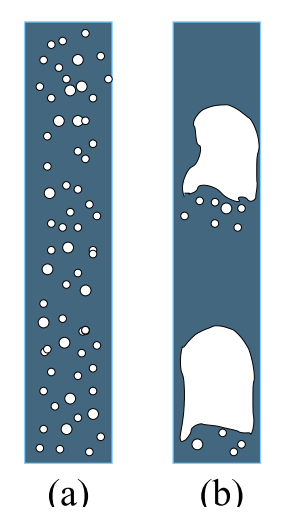
\includegraphics[scale=0.5]{regime.png}
    \caption{The two flow regimes in gas-liquid flow that is relevant in this thesis work \cite{Wetind2001}, (a) Bubbly flow, (b) Slug flow.}
    \label{regime}
\end{figure}


Gas-liquid two-phase flow can be classified into several categories \cite{Wetind2001}, in this work, we will focus on the bubbly flow regime. Bubbly flow exists with low volume fraction and low coalescence rate so that only small bubble forms. In bubbly flow, we can use the volume averaging approach Euler-Euler model, which will be discussed in the next section. However, according to \cite{Hine1980}, when the flow channel is narrow, and gas inlet flux is large, sufficient coalescence will lead to the formation of large bubbles as shown in figure \ref{regime}, (b), such flow regime is called slug flow. Since traditional volume averaging models are not suitable for the modelling of slug flow, we will avoid modelling slug flow by keeping the gas inlet flux low when the gap is less than $0.5 \,  \mathrm{cm}$.


\section{Numerical models for gas-liquid flow}
Multiphase flow model can be largely classified into two categories, the Euler-Lagrange model and the Euler-Euler model. In this study, we focus on the Euler-Euler model, as this model is cheaper and better implemented in commercial codes.


\subsection{The Euler-Euler model}\label{eemodel}
 In the Euler-Euler model, the continuous phase and dispersed phase are each solved by one set of Naiver-Stokes equation and mass transport equation:

\begin{equation}
    \frac{\partial \alpha_c}{\partial t} + \nabla \cdot (\alpha_c \mathbf{u_c}) = 0
\end{equation}

\begin{equation}
        \rho_c \frac{\partial (\alpha_c\mathbf{u_c})}{\partial t}  
        + \rho_c \nabla \cdot (\alpha _c \mathbf{u_c u_c}) + \alpha_c \nabla p + \nabla \cdot (\alpha_c \mathbf{τ_c} ) = \mathbf{M}
\end{equation}

\begin{equation}
    \mathbf{τ_c} = -\mu_c (\nabla \mathbf{u_c} + \nabla \mathbf{u_c}^T-\frac{2}{3}(\nabla \cdot \mathbf{u_c})\mathbf{I})
\end{equation}


\begin{equation}
    \frac{\partial \alpha_d}{\partial t} + \nabla \cdot (\alpha_d \mathbf{u_d}) = 0
\end{equation}

\begin{equation}
    \rho_d \frac{\partial (\alpha_d\mathbf{u_d})}{\partial t}  
        + \rho_d \nabla \cdot (\alpha _d \mathbf{u_d u_d}) + \alpha_d \nabla p + \nabla \cdot (\alpha_d \mathbf{τ_d} ) = -\mathbf{M}
\end{equation}

\begin{equation}
    \mathbf{τ_d} = -\mu_d (\nabla \mathbf{u_d} + \nabla \mathbf{u_d}^T-\frac{2}{3}(\nabla \cdot \mathbf{u_d})\mathbf{I})
\end{equation}

\begin{equation}
    \alpha_c+\alpha_d=1
\end{equation}

\begin{center}
\begin{tabular}{l l l| l l l}

  $\alpha_c$  &  continuous phase volume fraction & [$-$] & $\mathbf{u_c}$ & continuous phase velocity & [$\mathrm{m/s}$]\\
   
  $\mu_d$ & dispersed phase viscosity & [$ \mathrm{Pa \cdot s}$] & $\rho_c$ & continuous phase density & [$\mathrm{kg/m^3}$]\\
   
  $\mathbf{M}$ & interphase momentum transfer & [$\mathrm{N/m^3}$] & $\rho_d$ & dispersed phase density & [$\mathrm{kg/m^3}$]\\
   
  $p$ & operating pressure & [$\mathrm{Pa}$] & $\mu_c$ & continuous phase viscosity & [$\mathrm{Pa \cdot s}$]\\
   
  $\mathbf{u_d}$ & dispersed phase velocity & [$\mathrm{m/s}$] & 
  $\alpha_d$ & dispersed phase volume fraction & [-]
   
\end{tabular}
\end{center}

Note that all the velocities mentioned in this thesis are intrinsic velocities.

Solving both phases based on continuum description \cite{Darmana2005} means that we cannot see the detailed modelling of each bubble's motion, but this also makes the model cheaper, especially when there are many bubbles or discrete particles in the flow field.

 The two sets of Naiver-Stokes equations are coupled through the interphase momentum term $\mathbf{M}$. Since $\mathbf{M}$ is unknown, extra models need to be established to close these equations. This is accomplished by introducing empirical correlations. The interphase momentum transfer depends on various factors, which will be discussed in section \ref{bubblebehavior}.

\subsection{The mixture model}

The Euler-Euler model is widely used in industry for its relatively affordable computation cost. However, in early years, the two-way coupling through interphase momentum transfer could lead to severe convergence problem \cite{Sokolichin2004}. To overcome this problem, we sometimes neglect the influence of the dispersed phase on the continuous phase. However, in applications like bubble columns and airlift reactors, this means the liquid phase will be completely irrelevant. Another solution is to simplify the original equations by adding the momentum equations of both phase together:

\begin{equation}\label{eq:mix}
         \frac{\partial (\rho_c\alpha_c\mathbf{u_c}+\rho_d\alpha_d\mathbf{u_d})}{\partial t}  
        +  \nabla \cdot (\rho_c \alpha _c \mathbf{u_c u_c} + \rho_d \alpha _d \mathbf{u_d u_d})  + \nabla \cdot (\alpha_c \mathbf{τ_c} + \alpha_d \mathbf{τ_d}) + \nabla p
        = 0
\end{equation}

One of the two continuity equations could also be simplified by adding the two continuity equation together to eliminate the time derivative:

\begin{equation}
    \nabla \cdot (\alpha_c \mathbf{u_d}+\alpha_d \mathbf{u_c})=0
\end{equation}

One advantage of this simpler model is that the interphase momentum transfer is eliminated. However, as we can see, lacking one set of Navier-Stokes equation leads to the number of variables larger than the number of equations. Thus the model is not closed anymore. To solve this problem, we can rearrange the velocity into a term called mixture velocity $\mathbf{q}$:

\begin{equation}
    \mathbf{q}= \frac{\rho_c\alpha_c\mathbf{u_c}+\rho_d\alpha_d\mathbf{u_d}}{\rho_m}
\end{equation}

\begin{equation}
    \rho_m = \alpha_c \rho_c + \alpha_d \rho_d
\end{equation}

Furthermore, the continuous and dispersed phase velocity is coupled through a slip velocity:

\begin{equation}
    \mathbf{u_{slip}}=\mathbf{u_d} - \mathbf{u_c}
\end{equation}

The slip velocity is usually determined through force balance involved in the interaction between two phases. Although the calculation of slip velocity is physically similar to interphase momentum transfer in the full Euler-Euler model, it can usually be solved explicitly, which can reach convergence more easily when applied in the numerical model. The frequently used correlation for slip velocity will be discussed in the next section.

With the introduction of mixture velocity and slip velocity, we can rearrange equation \ref{eq:mix} into:

\begin{equation}
    \rho_m \frac{\partial \mathbf{q}}{\partial t} +\rho_m (\mathbf{q} \cdot \nabla )\mathbf{q} = -\nabla p -\nabla \cdot \mathbf{τ_m} - \rho_m \mathbf{g} - \nabla \cdot [\rho_m c_d (1-c_d)\mathbf{u_{slip}}\mathbf{u_{slip}}]
\end{equation}
   
   
\begin{equation}
    \mathbf{τ_m} = -\mu_m (\nabla \mathbf{q} + \nabla \mathbf{q}^T-\frac{2}{3}(\nabla \cdot \mathbf{q})\mathbf{I})
\end{equation}


\begin{equation}
    c_d = \frac{\alpha_d \rho_d}{\rho_m}
\end{equation}
The term $\mu_m$ is the mixture viscosity, dependent on the model chosen, a frequently used model proposed by Kreiger et al.\cite{Wedin2001} is:

\begin{equation}\label{eq:mixtureviscosity}
    \mu = \mu_d (1-\frac{\alpha_d}{\alpha_m})^{(-2.5\alpha_m[(\mu_d+0.4\mu_c)/(\mu_d+\mu_c)])}
\end{equation}

Where $
\alpha_m$ is the max packing volume fraction, whose value is based on empirical correlations.

Because of the use of mixture velocity, this simplified model is called the mixture model. This model is implemented in nearly all commercial and open-source codes \cite{COMSOL2013, ANSYSFLUENT13UsersGuide2013}.

\subsection{The bubbly flow model}\label{section:bubblyflowmodel}
In gas-liquid flow, the density of the dispersed phase is so much smaller than the continuous phase that it is acceptable to eliminate some terms involving gas density. Eliminating the term including $\rho_g$, we can obtain the further simplified version:

\begin{equation}\label{eq:bubbly1}
         \rho_c \frac{\partial (\alpha_c\mathbf{u_c})}{\partial t}  
        +  \rho_c \nabla \cdot (\alpha _c \mathbf{u_c u_c})  + \nabla \cdot (\alpha_c \mathbf{τ}) + \nabla p
        = 0
\end{equation}

\begin{equation}\label{eq:bubbly2}
    \mathbf{τ} = -\mu (\nabla \mathbf{u_c} + \nabla \mathbf{u_c}^T-\frac{2}{3}(\nabla \cdot \mathbf{u_c})\mathbf{I})
\end{equation}

With two sets of mass conservation equation, we complete the simplified bubbly flow model:

\begin{equation}\label{eq:bubbly3}
    \nabla \cdot (\alpha_d \mathbf{u_d} + \alpha_c \mathbf{u_c}) = 0
\end{equation}

\begin{equation}\label{eq:bubbly4}
    \frac{\partial \alpha_c}{ \partial t} + \nabla \cdot (\alpha_c \mathbf{u_c}) = 0
\end{equation}

The viscosity $\mu$ can be modelled based on a simplified version of equation \ref{eq:mixtureviscosity} by assuming $\alpha_m = 1$ and $\mu_d/\mu_c \approx 0$ \cite{ANSYSFLUENT13UsersGuide2013,Wedin2001}:

\begin{equation}\label{eq:bubbly5}
    \mu = \frac{\mu_c}{1-\alpha_d}
\end{equation}

\textbf{In this thesis work, we mainly used this model to study the bubbly flow behaviour.}

\subsection{ Turbulence model in bubbly flow}\label{turbulentmodel}

Standard $k-\varepsilon$ model with extra source-term in the dissipation rate transport equation is employed to model the bubbly flow \cite{COMSOL2016}:

\begin{equation}
    \mathbf{τ_c} = -(\mu + \mu _T) (\nabla \mathbf{u_c} + \nabla \mathbf{u_c}^T-\frac{2}{3}(\nabla \cdot \mathbf{u_c})\mathbf{I})
\end{equation}

\begin{equation}
    \mu_T = 0.09 \rho_c \frac{k^2}{\varepsilon}
\end{equation}

\begin{equation}
    \rho_c \frac{\partial k}{\partial t} + \rho_c (\mathbf{u_c} \cdot \nabla) k = \nabla \cdot [(\mu + \mu_T /\sigma_k)\nabla k] + P_k - \rho_c \varepsilon +S_k
\end{equation}

\begin{equation}
    \rho_c \frac{\partial \varepsilon}{\partial t} + \rho_c (\mathbf{u_c} \cdot \nabla) \varepsilon = \nabla \cdot [(\mu + \mu_T /\sigma_{\varepsilon})\nabla \varepsilon] + C_{\varepsilon1} \frac{\varepsilon}{k} P_k - C_{\varepsilon2} \rho_c \frac{\varepsilon^2}{k} + C_{\varepsilon} S_k \frac{\varepsilon}{k}
\end{equation}

\begin{equation}
    S_k = -C_k \alpha_d \nabla p \cdot \mathbf{u_{slip}}
\end{equation}

\begin{center}
\begin{tabular}{l l l| l l l}

  $k$  &  Turbulent kinetic energy & [$\mathrm{m^2/s^2}$] & $\varepsilon$ & Dissipation rate & [$\mathrm{m^2/s^3}$]\\
   
  $\mu_T$ & eddy viscosity & [$ \mathrm{Pa \cdot s}$]
   
\end{tabular}
\end{center}

$S_k$ is the extra source term, also known as bubble-induced turbulence \cite{Rzehak2013}, and $\sigma_k, P_{\varepsilon}, S_k, C_{\varepsilon 1}, C_{\varepsilon 2}, C_{\varepsilon}, C_k$ are all empirical parameters from standard $k-\varepsilon$ model \cite{COMSOL2016}.

\subsection{The Stokes number criteria}\label{stokessection}

In the previous section, we have walked through the simplification process from the full Euler-Euler model  to the Bubbly flow model. Based on \cite{ANSYSFLUENT13UsersGuide2013}, there is a general criterion deciding whether a model is applicable for a case, and the criterion is based on the Stokes number $\mathrm{St}$:

\begin{equation}
    \mathrm{St} = \frac{\tau_d}{t_s}
\end{equation}

\begin{equation}
    \tau_d = \frac{\rho_d D_e^2}{18 \mu_c}
\end{equation}

\begin{equation}
    t_s = \frac{L_s}{V_s}
\end{equation}

$L_s$ and $V_s$ represent the characteristic length and velocity. 

When $\mathrm{St} \ll 1$ or $\mathrm{St} \approx 1$, any of the model introduced above can be chosen, when $\mathrm{St} >1$, the particles or bubbles move independently of the flow, mixture model or bubbly flow is not applicable anymore.

For the case in this study, $t_s \approx 0.1 \, \mathrm{s}$, $\tau \approx 10^{-17}$, $St = \tau_d / t_s \approx 10^{-16}$, therefore, bubbly flow model is applicable.


\section{Bubble behaviors}\label{bubblebehavior}

In this section, the properties of bubbles will be discussed. A series of empirical correlations used for closing the model discussed in the previous section will be presented.

\subsection{Single bubble properties}

In 1987, Clift \cite{clift1978bubbles} treated the behaviour and shape of bubbles as a function of several relevant dimensionless numbers


The relevant dimensionless numbers mentioned by Clift are Reynolds number, Eötvös number, and Archimedes number; their expression is shown below:

\begin{equation}
   \mathrm{Re} = \frac{\rho |\mathbf{u_{slip}}| L}{\mu_c}
\end{equation}

\begin{equation}
    \mathrm{Eo} = \frac{\Delta \rho g L^2}{\gamma}
\end{equation}

\begin{equation}
    \mathrm{Ar} = \frac{gL^3\rho_c \Delta \rho}{\mu_c^2}
\end{equation}

$\gamma$ stands for surface tension coefficient.

The involvement of these three dimensionless numbers implies that the major forces influencing the bubble behaviour are the buoyancy force, the surface tension force, inertial force and viscous force.

For tiny bubbles with a diameter less than $1 \, \mathrm{mm}$, we usually have $ \mathrm{Eo} \ll 1$, in this case, the bubble has a spherical shape, and the bubble velocity is solely dependent on the Archimedes number \cite{batchelor2000introduction}. Therefore, surface tension force can be neglected, and the force balance of a single bubble can be rearranged as:
\begin{equation}
    |\rho_c-\rho_d|g\frac{\pi D_e ^3}{6}=C_d\frac{\pi D_e^2}{4}\cdot \frac{1}{2}\rho_c | \mathbf{ u_{slip}} |^2
\end{equation}
Where $D_e$ is the bubble diameter, as shown in figure \ref{force}.

\begin{figure}[H]
    \centering
    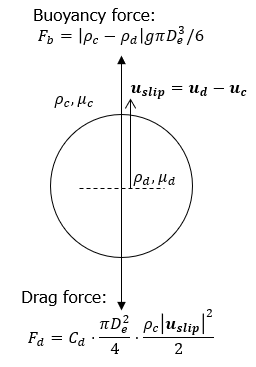
\includegraphics{force_balance.png}
    \caption{Force balance between buoyancy force and drag force for a single small spherical bubble}
    \label{force}
\end{figure}

In this way, we transform the problem into a relatively simple model; the remaining variables that need to be filled are the bubble diameter and drag force coefficient $C_d$. Information about these two terms can both be found in various literature through history. It is also worth to know that \textbf{Small spherical bubbles are also the focus of this thesis work}, as they usually exist in the electrochemical cell \cite{Energy}.

\subsection{Drag models}\label{section:dragmodel}
The frequently used drag model is the Schiller-Naumann model \cite{schwarzkopf2011multiphase}:

\begin{equation}
  C_d=\begin{cases}
               \frac{24}{\mathrm{Re_p}}(1+0.15\mathrm{Re_p}^{0.678}), \quad \mathrm{Re_p} <1000\\
               0.44, \quad \mathrm{Re_p}>1000
            \end{cases}
\end{equation}

Schiller-Naumann model is appropriate for dilute flows since the correlation is based on a single bubble and does not take bubble-bubble interaction into account \cite{COMSOL2016}.

When dealing with bubble swarm, however, we need to consider the interaction between the bubbles. Wen and Yu proposed a corrected model based on the existing Schiller-Naumann model:

\begin{equation}\label{eq:wenyudrag}
  C_d=\begin{cases}
                \frac{24}{\mathrm{Re_p}}\alpha_d^{-2.65}, \quad \mathrm{Re_p}<0.5 \\
               \frac{24}{\mathrm{Re_p}}(1+0.15\mathrm{Re_p}^{0.678}) \alpha_d^{-2.65}, \quad 0.5<\mathrm{Re_p} <1000\\
               0.44\alpha_d^{-2.65}, \quad \mathrm{Re_p}>1000
        \end{cases}
\end{equation}

where $\mathrm{Re_p}$ is the particle(bubble) Reynolds number


When the particle Reynolds number is less than one, Stokes drag law is also valid:

\begin{equation}
    C_d = \frac{24}{\mathrm{Re_p}}
\end{equation}
% An extended correlation is also given by \cite{Energy}:

% \begin{equation}
%     C_d = \frac{16}{\mathrm{Re_p}}+\frac{14.9}{\mathrm{Re_p}^{0.78}(1+10\mathrm{Re_p}^{-0.6})}
% \end{equation}

% which is valid for:
% \begin{equation}
%     \mathrm{Re_p}<2.3(\frac{\gamma^3}{g\nu^4_L\rho^3_L})^{0.209}
% \end{equation}

% This correlation does not have a definite range, but it is claimed in \cite{Energy} that it is suitable when the deformation of bubbles is negligible.

\subsection{The implementation of drag models in momentum equations}

The implementations of these drag models in the Euler-Euler and mixture model are slightly different. In the Euler-Euler model, the drag model is directly incorporated into the interphase momentum transfer $\mathbf{M}$ \cite{oliveira2003numerical}, from figure \ref{force} we know that the drag force applied on a single particle can be written as:

\begin{equation}
    \mathbf{F_D} = \frac{\pi D_e^2}{4} \frac{\rho_c C_d |\mathbf{u_{slip}}| \mathbf{u_{slip}}}{2}
\end{equation}

While the implemented interphase momentum transfer is the drag force per computation cell, which can be written as:

\begin{equation}\label{eq:interphase_momentum}
    \mathbf{M} = \frac{\mathbf{F_D}}{V_{bubble}} \cdot \frac{V_{bubble}}{V_{cell}}
\end{equation}

Where $V_{bubble} = \frac{\pi D_e^3}{6}$ is the volume of a single bubble, $V_{cell}$ is the volume of a single computation cell, with $\alpha_d \equiv \frac{V_{bubble}}{V_{cell}}$, substitute it into equation \ref{eq:interphase_momentum} we get:

\begin{equation}\label{eq: particle model}
    \mathbf{M} = \frac{3}{4D_e}\alpha_d C_d \rho_c |\mathbf{u_{slip}}|\mathbf{u_{slip}}
\end{equation}

This is the interphase momentum transfer based on particle model. One drawback of this model is that when the volume fraction of gas reaches one, the interphase momentum still exists, while in reality, it should disappear, so a corrected symmetrical model is more frequently used \cite{ANSYSFLUENT13UsersGuide2013}:

\begin{equation}\label{eq:balance}
    \mathbf{M_{sym}} = \frac{3}{4D_e}\alpha_d\alpha_c C_d \rho_c |\mathbf{u_{slip}}|\mathbf{u_{slip}}
\end{equation}

This is the most frequently used form of interphase momentum transfer in the Euler-Euler model.

In the mixture model, however, it is slightly different, since the momentum equations of mixture model do not have the interphase momentum transfer term. In bubbly flow, a force balance between pressure force and drag force based on slip velocity is used \cite{kuzmin2000efficient}:

\begin{equation}
    -\alpha_d \nabla p = \mathbf{M}
\end{equation}

On the left-hand side is the pressure force of the bubbles in each computation cell. On the right-hand side is the interphase momentum transfer based on particle model from equation \ref{eq: particle model}, here we used particle model instead of symmetrical model equation \ref{eq:balance} because using the former one can help us explicitly solve the slip model.


Additionally, it is essential to note that this force balance is based on the assumption that the bubbles reach its terminal velocity instantly so the acceleration term can be terminated. From the discussion in section \ref{stokessection}, we know that this assumption is valid here.

% The force balance of a particle in fluid can be written in the below form\cite{Sokolichin2004}:

% \begin{equation}\label{eq:time}
%     m \frac
%     {d \mathbf{u_{slip}}}{dt} = \mathbf{F} - \frac{\mathbf{u_{slip}}}{C}
% \end{equation}

% Where $m$ is the mass of a single bubble
% The solution of this equation can be written as:

% \begin{equation}\label{eq:solution}
%     \mathbf{u_{slip}}(t) = C\mathbf{F}(1-e^{-t/(mC)}) 
% \end{equation}

% From equation \ref{eq:solution} we can see that the time a single particle spent reaching steady-state scales with $mC$. Because the mass of gas bubbles is extremely small, for example for a $100 \mu m$ hydrogen bubble $ m \approx 5 \times 10^{-14}$ kg, and $C \approx 4 \times 10^7 s/kg$ \cite{Sokolichin2004}. The time for this bubble to reach steady state is at the same magnitude with $ \tau = mC \approx 10^{-6} s$. Therefore, it is valid to assume that small spherical gas bubbles reach steady-state instantly.

Now if we substitute the Stokes drag law into equation \ref{eq:balance}, the slip velocity can be explicitly solved:

\begin{equation} \label{eq:slip}
    \mathbf{u_{slip}} = \frac{\nabla p D_e^2}{12\mu}
\end{equation}

Under the assumption that the total pressure gradient can be approximated by hydrostatic pressure gradient \cite{Sokolichin2004}:

\begin{equation}
    \nabla p \approx \rho_c \mathbf{g}
\end{equation}

Substitute it into equation \ref{eq:slip}, we get:

\begin{equation}\label{eq:stokes_slip}
    \mathbf{u_{Stokes}} = \frac{\rho_c D_e^2 \mathbf{g}}{18\mu}
\end{equation}

This is the Stokes slip velocity.

\subsection{Other forces}\label{otherforces}

The drag force is the most important force, but sometimes there are also other forces included in the interphase momentum transfer term $\mathbf{M}$, or the force balance equation of the mixture model. 

\paragraph{Lift force}
\*

\begin{figure}[H]
    \centering
    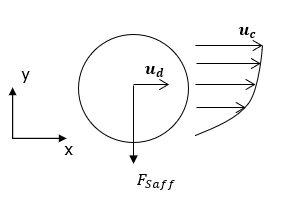
\includegraphics{saffman.png}
    \caption{A sketch for Saffman lift force, when the liquid phase shear rate $du_{cx}/dy>0$, and $\mathbf{u_c}<\mathbf{u_d}$, the Saffman lift force points downwards}
    \label{Saffman}
\end{figure}

When a sphere moving through viscous liquid, it experiences a lift force \cite{saffman1965lift}:

\begin{equation}\label{eq:lift}
    \mathbf{ F_{Saff} } = 1.615 \rho_c \nu_c^{1/2} D_e^2 (u_{dx} - u_{cx})|\frac{d u_{cx}}{d y}|\mathrm{sign}(\frac{d u_{cx}}{d y})\mathbf{e_y}
\end{equation}

Note that the Lift force here is normal to the direction of the velocity. When implemented in the context of buoyancy-driven flow, the major velocity is in the y-direction, thus the direction of the lift force is in the x-direction instead. Additionally, to simplify the model, we can use the stokes slip velocity from equation \ref{eq:stokes_slip} as the velocity term:

\begin{equation}
    u_{dy} - u_{cy} \approx |\mathbf{u_{Stokes}}|
\end{equation}

This is true because stokes slip velocity counts more than 90% of the slip velocity on y direction based on simulation results \cite{Schillings2015}. Therefore, equation \ref{eq:lift} can be rearranged into:

\begin{equation}\label{eq:saff}
    \mathbf{ F_{Saff} } = 1.615 \rho_c \nu_c^{1/2} D_e^2 |\mathbf{u_{Stokes}}| |\frac{d u_{cy}}{d x}|^{0.5} \mathrm{sign}(\frac{d u_{cy}}{d x})\mathbf{e_x}
\end{equation}

To implement it in the bubbly flow model, we need to balance it with drag force:

\begin{equation}
    \mathbf{F_{Saff}} = C_d \frac{\pi D_e^2}{4} \frac{\rho_c |\mathbf{u_{slip}} |^2}{2} 
    = \frac{16 \mu_c }{\rho_c \mathbf{u_{slip}} D_e} \frac{\pi D_e^2}{4} \frac{\rho_c |\mathbf{u_{slip}}| ^2}{2}
\end{equation}

Substitute into equation \ref{eq:saff}, we can directly solve the Saffman lift velocity:

\begin{equation}\label{eq:Saff}
    \mathbf{u_{Saff}} = 0.257 D_e \mathrm{sign}(\frac{d u_{cy}}{d x}) |\frac{d u_{cy}}{d x}|^{0.5} \nu_c^{-0.5} |\mathbf{u_{Stokes}}| \mathbf{e_x}
\end{equation}

\paragraph{Diffusion}
\*

Small spherical bubbles in electrochemical cells behave like small particles in sedimentation process \cite{Dahlkild2001}, Wedin et al. \cite{Wetind2001} summarise the diffusion and migration behavior from various literature \cite{nicolai1995particle, schaflinger1990centrifugal, leighton1987measurement}, and give the empirical formula in the form of slip velocity:

\begin{equation}\label{eq:diffusion}
    \mathbf{ u_{diffusion} } = \big( -\frac{D_e |\mathbf{u_{Stokes}}|}{2} \mathcal{D} - D_e^2 |\frac{d u_{cx}}{d y}| \frac{\alpha_d (1 + 0.5 e^{8.8 \alpha_d})}{12} \big) \frac{\nabla \alpha_d}{\alpha_d (1 - \alpha_d)}
\end{equation}

Where $\mathcal{D}$ is the Dimensionless coefficient matrix in diagonal form \cite{nicolai1995particle}: 

\begin{equation} 
\mathcal{D} = \begin{pmatrix}1 & 0\\ 0 & 8\end{pmatrix}
\end{equation}


In equation \ref{eq:diffusion}, there are two terms. The first term comes from hydrodynamic self-diffusion, according to \cite{nicolai1995particle}, during the settling of non-Brownian spheres, the particle motion is demonstrated to be diffusive. Through experiments, they proposed a volume fraction diffusion term based on Stokes slip velocity. The second term comes from shear-induced self-diffusion \cite{schaflinger1990centrifugal}, which is a volume fraction diffusion term based on shear rate.

\paragraph{Added mass force}
\*

If the bubble accelerated in a uniform flow field, it experiences an extra force since the fluid around the bubble has to be accelerated as well \cite{kundu2015fluid}. The accelerated fluid is the added mass, and this additional force is the added mass force. It can be written as \cite{Darmana2005}:

\begin{equation}
    \mathbf{ F_{am} } = \rho_c C_{am} V_{bubble} \frac{d\mathbf{u_{slip}}}{dt}
\end{equation}

Where the coefficient $C_{am}$ relates to the local volume fraction of gas, according to \cite{Sokolichin2004}, it is rather difficult to estimate the value of $C_{am}$ accurately, but from section \ref{stokessection} we know that the time for small spherical bubbles in electrochemical cells to reach its terminal velocity is extremely short. Therefore, it is safe to neglect the added mass force in this case.

\paragraph{Turbulent dispersion force}
\*

In bubbly flow, the turbulent dispersion force is modelled in the form of an extra drift velocity term \cite{Sokolichin2004}:

\begin{equation}
    \mathbf{u_d} - \mathbf{u_c} = \mathbf{u_{slip}} + \mathbf{u_{drift}}
\end{equation}

\begin{equation}\label{eq:drift}
    \mathbf{u_{drift}} = -\mu_T \frac{\nabla \alpha_d}{\rho_c \alpha_d}
\end{equation}

We can see a similar form between the turbulent dispersion and diffusion, they both include the term $\frac{\nabla \alpha_d}{\alpha_d}$, which can be interpreted as volume fraction diffusion with diffusion coefficients.

Based on Ruzicka et al. \cite{Ruzicka2003} and Schilling et al. \cite{Schillings2015}, we can balance the diffusion term with the convection term in the transport equation of volume fraction \cite{Schillings2015}: 

\begin{equation}\label{convectiondiffusion}
     \mathbf{u_c} \cdot \nabla \alpha_d = \nabla(\alpha_c \mathbf{u_{slip}})
\end{equation}

substitute equation \ref{eq:drift} and \label{eq:diffusion} into \ref{convectiondiffusion} we get the form:

\begin{equation}
    \nabla \cdot (\mathbf{u_c} \alpha_d) = -\mathcal{D_{\alpha}} \nabla^2 \alpha_d 
\end{equation}

$\mathcal{D_{\alpha}}$ is the coefficient lumping the coefficients of all the slip velocity terms that involve the volume fraction gradient, it can be interpreted as the volume fraction diffusion coefficient, though it is a field dependent variable similar to eddy viscosity.


\subsection{Swarm effects in electrochemical cells}

In section \ref{section:dragmodel}, we have already seen the correction term $\alpha^{-2.65}_d$ in the Wen-Yu drag model. This is called the hindrance function, used for describing the particle or bubble interaction when the dispersed phase concentration is high enough.

In electrochemical cells, there are also specific hindrance functions describing the bubble swarm behaviour, despite the similarity between the gas-evolving electrochemical cells and traditional bubble columns. The main differences between bubbles in electrochemical cells and in normal reactors are that the gas bubbles in electrolyte solutions usually have a surface charge that can impact the interaction between themselves. In water electrolysis, for instance, usually $\mathrm{KOH}$ solution is used as the electrolyte, which means the concentration of $\mathrm{OH^-}$ is high. Such a high concentration of $\mathrm{OH^-}$ will cause a lot of them to attach to the surface of bubbles, which creates electrostatic repulsion between bubbles and prevents coalescence \cite{Kreysa1985}. Therefore, certain corrected models describe the bubble swarm model as the coalescence barrier are model proposed.

The Richardson-Zaki equation gives a decent approximation of the bubble swarm rising velocity \cite{richardson1954sedimentation}:

\begin{equation}\label{eq:richardson}
    u_{swarm} = (1-\alpha_d)^{4.65} u_{single}
\end{equation}

$u_{single}$ is the single bubble rise velocity relative to the liquid velocity, this equation is widely used for various applications, not limited to electrochemical cells. This approximation works well when the volume fraction is less than 0.3, later Marucci developed an alternative hindrance function, which provides better approximation at higher volume fraction \cite{wendt1999electrochemical}:

\begin{equation}
    u_{swarm} =\frac{(1-\alpha_d)^2}{1-\alpha_d^{5/3}}  u_{single}
\end{equation}

Kreysa \cite{Kreysa1985} derived the coalescence barrier model based on the swarm velocity:

\begin{equation}
   \alpha_d = \frac{\alpha_m \alpha_d u_d}{\alpha_d u_d+u_c(\alpha_m-\alpha_g)+u_{swarm}\alpha_d}
\end{equation}

This model is developed exclusively for the bubble interaction in electrochemical cells. $\alpha_m$ is the maximum the gas volume fraction, an empirical value. This equation can be rearranged into the form of slip velocity:

\begin{equation}\label{eq:coalescencebarrier}
    u_{slipy}(1-\frac{\alpha_d}{\alpha_m}) = u_{swarm}
\end{equation}

The same equation could be derived from Vogt's correlation in \cite{Energy}. Please note that here the velocities are all scalar since only the rise velocity is considered. 

In the testing of various slip models in this thesis work, it is found that the coalescence barrier model in equation \ref{eq:coalescencebarrier} could cause the solver to crash, once the $\alpha_m$ is too small or the current density is too large. 



\section{Bubbly flow in electrochemical cells}

In the previous sections, the basic hydrodynamics theory has been introduced. In this section, we will discuss bubble behaviour in the electrochemical cell, including the basic electrochemistry theory, its simplification in the model, and the theory that lays the foundation for the model used in this thesis study.

\subsection{Bubble nucleation}

One of the differences between bubbly flow in normal channels and electrochemical cells is the bubble nucleation process. Usually, in normal two-phase reactors bubbles are injected into the container, but the in electrochemical cells bubble is directly generated from the electrode. Sometimes the electrode could be a plate, which makes the bubble generation a boundary condition. Sometimes when the porous electrodes are involved, the bubble generation then becomes a source term \cite{charton2009hydrogen}.

For the bubble nucleation on a plate electrode, Wüthrich et al. gives a good diagram \cite{Wuthrich2015, L.J.J.Janssen1988}:

\begin{figure}[H]
    \centering
    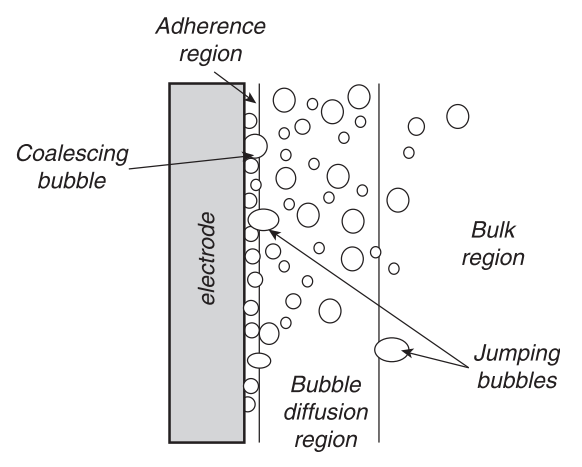
\includegraphics{nucleation.png}
    \caption{Bubble nucleation process on a plate electrode \cite{Wuthrich2015}}
    \label{nucleation}
\end{figure}

where the bubbles near the electrodes have a structure of three regions:

\begin{enumerate}[(a)]
    \item Adherence region: Bubbles in the adherence region are first produced at certain sites of cracks on the electrode surface;
    \item Bubble diffusion region: Bubbles keep growing in the Adherence region until they reach a certain size, a critical radius whose correlation can be found in \cite{Energy}, they diffuse into the bubble diffusion region. This region has high bubble concentration; sometimes they are called bubble curtain or plume from literature \cite{Balzer2002, Darmana2005}, this bubble layer usually has several millimetres;
    \item Bulk region: In the bulk region, only a few dispersed bubbles exist. The size of the bulk region depends on the reactor size; sometimes for narrow containers like the channel studied in this thesis work, the bulk region could be relatively small. 
\end{enumerate}

One of the challenges in bubble nucleation is the lack of information for volume fraction in the adherence region \cite{Alexiadis2011, Alexiadis2012, Alexiadis2012a, Alexiadis2012b}. Balzer et al. \cite{Balzer2002} derived a correlation between the bubble coverage on the electrode surface and flow velocity. Nevertheless, bubble coverage on the surface is still different from the bubble volume fraction in the near-wall region; it is expected that a submodel can be derived in this region based on experimental data, but due to extremely small size of this region, reliable experimental data have not been found yet \cite{Hreiz2015}. 

Therefore, the modelling of adherence region will be simplified in this work; the bubble nucleation process will be modelled as injection instead. It means the main focus of the modelling work will be on the bubble diffusion region. However, the problem of unknown volume fraction at the boundary still remains. In simulation works from literature, the value of volume fraction is either assumes \cite{Alexiadis2011, Alexiadis2012, Alexiadis2012a, Alexiadis2012b}, or obtained directly from the experiment (for relatively wide channels) \cite{Mat2005}.

While the Euler-Euler model requires both velocity and volume fraction as the input parameter as a boundary condition, the mixture model only requires the flux:
\begin{equation}\label{eq:gasflux}
    N_{gas} = \alpha_d u_{dx}
\end{equation}

In this way the problem of unknown volume fraction problem is bypassed, the mixture model can solve the volume fraction at the region iteratively, though it does not mean the value obtained is physically true, more experiment works are still required \cite{Alexiadis2012}.

\subsection{Simplification of the electrochemistry part}

% One idea for studying the phenomena could be building a advanced model including the all three aspects as well as the coupling between them, Hreiz et al. \cite{Hreiz2015} gave a good illustration of the coupling between different physics in figure \ref{couple}:

% \begin{figure}[H]
%     \centering
%     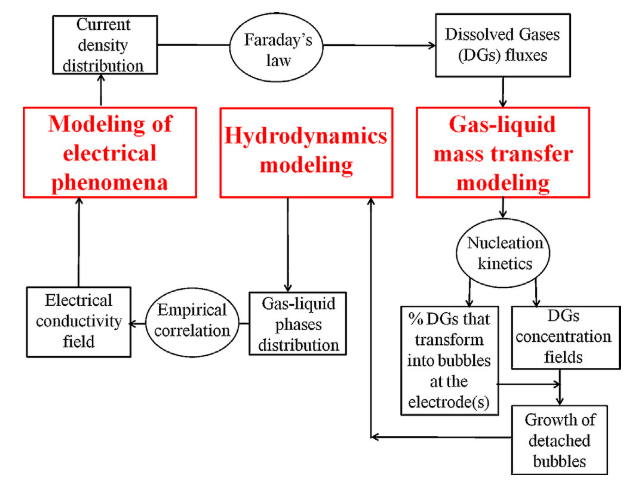
\includegraphics{coupling.png}
%     \caption{Coupling between different physics \cite{Hreiz2015}.}
%     \label{couple}
% \end{figure}

% As we can see, these are very complex interactions. Darmana et al. \cite{Darmana2005} proposed an advanced model including all the factors mentioned above under the framework of Euler-Lagrange. However, as discussed in the previous section, the Euler-Lagrange model is not available in any commercial code yet, in OpenFOAM it is not readily available either, but only accessible through manually coupling the interFOAM and solidParticle library.

% More recently, there are works treating similar problems under the framework of Euler-Euler model combined with Population balance model \cite{Askari2018, Buffo2017}, in this way the bubble diameter distribution could be included through solving an extra set of bubble number density function, even if the Euler-Euler model applies volume average for the dispersed phase.

The coupling between different physics in elctrochemical cells are complex and highly interdependent, simplifications are made on different levels \cite{Hreiz2015} in most of the literature. To study the phenomena we are interested, the hydrodynamic effect, we also avoided the modelling of mass transfer and electrical phenomena. The influences of these phenomena on the hydrodynamics are modelled through empirical correlations from literature instead.


% From figure \ref{couple} we can see the most important coupling mechanism involving the hydrodynamics part is the growth of detached bubbles. 

The bubble evolution process is simplified as bubble injection, and to model this part we can derive the relation between the current density and the inlet gas flux based on mass balance and ideal gas law \cite{Energy}:

\begin{equation}\label{eq:gasevolution}
    N_{gas} = \frac{RTi_{av}}{npF}
\end{equation}

$R$ is the ideal gas coefficient, $F$ is the Faraday constant, $p$ is the operating pressure, $i_{av}$ is the average current density along with the electrode plate, $T$ is the temperature, and $n$ is the number of electrons transferred in one molecule of gas. In the reaction we study:

\begin{equation}\label{eq:currentdensity}
2\mathrm{H_2O} + 2e^- \longrightarrow \mathrm{H_2} + \mathrm{OH^-}
\end{equation}

the number of electrons transferred is two, so $n = 2$.

With equation \ref{eq:currentdensity}, we can determine the inlet gas flux by entering a reasonable current density.


\section{Literature review}

In this section, we will introduce some simulations and experimental works from the literature that inspire this thesis work.

\subsection{Modeling works}\label{modellingreview}

The modelling works could be largely classified into the simulation in the natural flow, where there is no liquid phase inlet velocity applied on the boundary, and forced flow, where a liquid phase inlet velocity is given. 

\paragraph{Natural flow}
\*

Iga et al. \cite{K.IGAand} developed a 2D multiphase flow model using one set of Naiver-Stokes equation given by \cite{matsumoto1991numerical}. The model describes the bubble rise in a horizontal quiescent channel, and it is observed that plumes of bubble contained fluid are produced by Raleigh-Taylor instability, and the convective patterns mainly depend on the gas phase superficial velocity and the volume fraction. Climent et al. \cite{Climent1999} modelled a similar case based on spatially filtered Naiver-Stokes equation, and found the counter-rotating structures induced by Raleigh-Taylor instability, as shown in figure \ref{rotating}:

\begin{figure}[H]
    \centering
    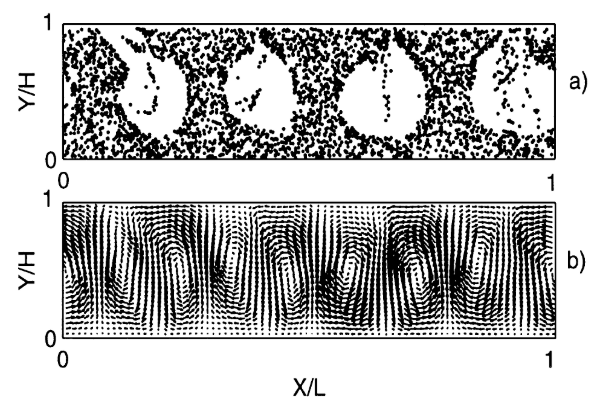
\includegraphics[scale = 0.75]{rotating.png}
    \caption{Counter-rotating structure \cite{Climent1999}, vortices form in the horizontal channel and the vortices near each other rotates in the opposite direction}
    \label{rotating}
\end{figure}

Later, Alexiadis et al. \cite{Alexiadis2011, Alexiadis2012, Alexiadis2012a, Alexiadis2012b} built a full Euler-Euler model in a vertical quiescent channel, the similar instability phenomena are observed, as shown in figure \ref{pseudo}:

\begin{figure}[H]
    \centering
    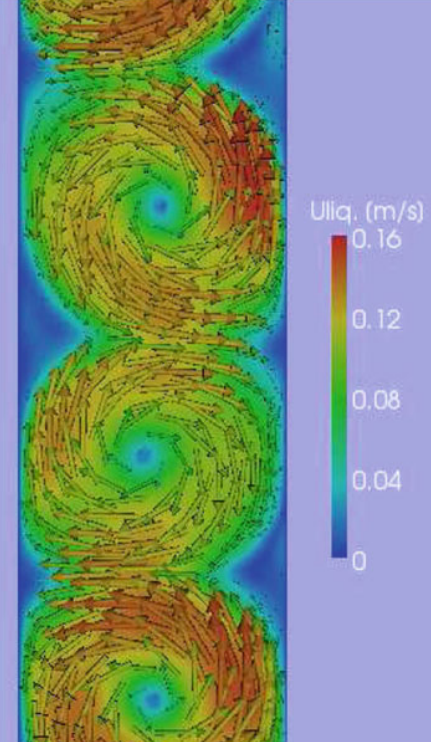
\includegraphics[scale=0.4]{vertical_rotating.png}
    \caption{pseudo turbulent structure in vertical channel \cite{Alexiadis2012}, the vortices near each other rotates in the opposite direction}
    \label{pseudo}
\end{figure}

It is called the pseudo-turbulence in the paper; the author also derived a criterion for the transition of flow field from steady-state to pseudo-turbulent state \cite{Alexiadis2012} based on a new dimensionless number:

\begin{equation}\label{ptcriterion}
    \Delta = \frac{N_{gas}\nu_c^{1/3}}{D_e^4h^2g^{7/3}}
\end{equation}

Where $h$ is the channel gap size, $N_{gas}$ is the inlet gas flux, and $\nu_c$ is the liquid phase kinematic viscosity. According to Alexiadius, the flow transits to pseudo-turbulence as the dimensionless number $\Delta$ increases. This means with smaller bubble size and larger gas inlet flux in a narrower channel; the flow tends to transit to pseudo-turbulence. In their study, for a $3 \, \mathrm{mm}$ channel, under gas flux of $N_{gas} = 1.5 \times 10^{-4} \, \mathrm{m/s}$ (based on equation \ref{eq:gasflux} this means the fed current density is around $1200 \, \mathrm{A/m^2}$), pseudo turbulence emerges when the bubble diameter surpasses $15 \, \mathrm{μm}$

While this instability phenomenon was found in quiescent channels, for the circulating channel of certain geometry, vortices were also observed in the simulations of circulating channels, more discussions can be found in Appendix \ref{appendixa}.

Besides the transition to pseudo-turbulence, Alexiadius et al. also provide the volume fraction profile in quiescent channels:

\begin{figure}[H]
    \centering
    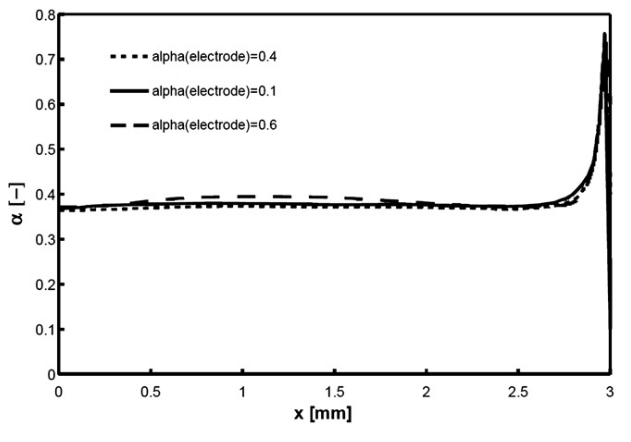
\includegraphics[scale=0.6]{volumefractionprofile.png}
    \caption{volume fraction profile in a quiescent channel with different assumed volume fraction value at the electrode surface \cite{Alexiadis2012}, different assumed number did not make large differences to the volume fraction profile, while certain amounts of bubble were trapped in the channel.}
    \label{volumefraction}
\end{figure}


% An Euler-Euler model including the energy equation was developed in PHOENICS by Agranat et al.\cite{agranat2006cfd}, while a similar model including the Nernst-Planck equation was developed by Mat et al. \cite{Mat2005}, they also studied a vertical quiescent channel. Although Mat et al. used the Euler-Euler model, no information about the inlet gas volume fraction was given, which is in conflict with the problem raised by Alexiadis \cite{Alexiadis2011a}, it is likely that they directly used the experiment data as the model input. 

At nearly the same time, Philippe et al. \cite{philippe2005modelling} proposed a Euler-Lagrange model coupled with an electrical model in a quiescent channel. The volume fraction profile in the channel is given in their work, shown in figure \ref{lagrangianplume}. One striking difference between the two subfigures shown below is that the bubble plume thickness grows with height when $D_e = 1 \, \mathrm{mm}$, but becomes independent of height when $D_e = 0.1 \mathrm{mm}$.
\begin{figure}[H]
    \centering
    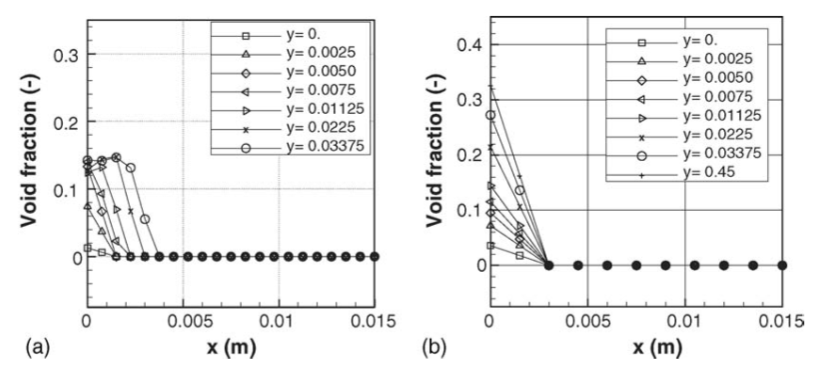
\includegraphics[scale=0.7]{volumeprofile.png}
    \caption{volume fraction profile in vertical quiescent channel \cite{philippe2005modelling}, x is on the channel width direction, y is on the channel height direction, the diagram gives volume fraction profile at different height of the channel, average current density is $4000 \, \mathrm{ A/m^2}$. Left: bubble diameter = $10^{-3}\, \mathrm{m}$. Right: bubble diameter = $10^{-4} \, \mathrm{m}$}
    \label{lagrangianplume}
\end{figure}

% They also tried adding a dispersion force to the horizontal direction, and gave the influences the force have on the bubble plume thickness in figure :

% \begin{figure}[H]
%     \centering
%     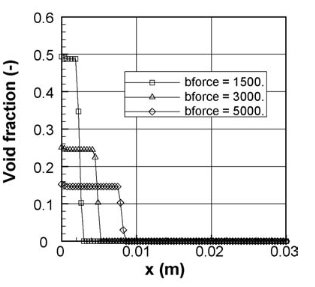
\includegraphics[scale=0.9]{horizontalforce.png}
%     \caption{The influences of adding a horizontal force with different magnitude \cite{philippe2005modelling}, bforce in the diagram refers to the dispersion force added on the horizontal direction}
%     \label{horizontalforce}
% \end{figure}

Abdelouahed et al. \cite{abdelouahed2014hydrodynamics}  adopted a Euler-Euler model to study natural channel flow.




\begin{figure}[H]
    \centering
    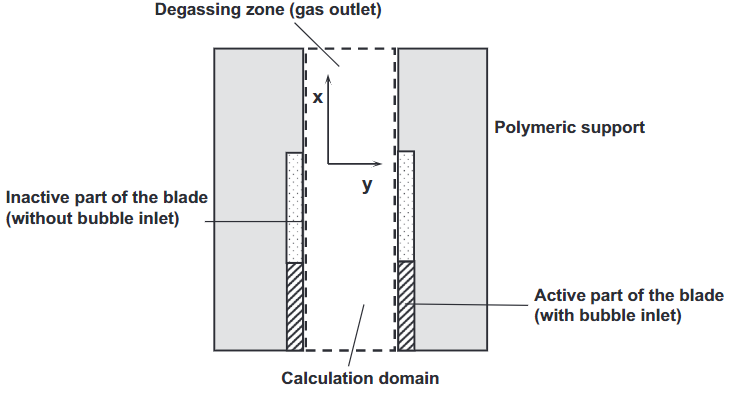
\includegraphics[scale=0.5]{lantern.png}
    \caption{Vertical quiescent channel \cite{abdelouahed2014hydrodynamics}, the channel width is $6 \, \mathrm{mm}$}
    \label{lantern}
\end{figure}

In their model, no inlet velocity at the bottom is given; thus, it is a quiescent channel similar to the one studied by Alexiadius et al. The volume fraction distribution in the channel is given.

\begin{figure}[H]
    \centering
    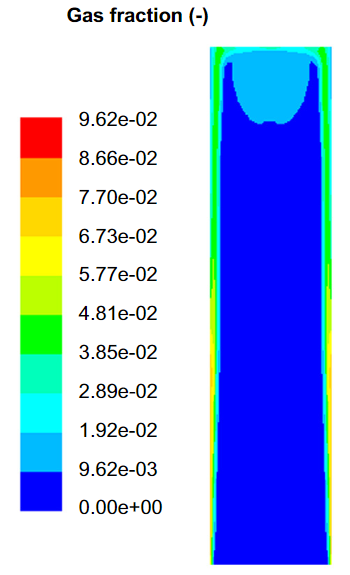
\includegraphics[scale=0.4]{volumedistribution.png}
    \caption{2D volume fraction distribution in a $6 \, \mathrm{mm}$ quiescent channel \cite{abdelouahed2014hydrodynamics}, current density is $1000 \, \mathrm{A/m^2}$ }
    \label{volumedistributionlag}
\end{figure}

From the diagram, we can see that the bubble plume is quite thin, which also matches well with their experiment mentioned in figure \ref{bubblephoto}.

Wedin et al. \cite{Wedin2001} proposed a mixture model developed in CFX describing the buoyancy-driven flow between two vertical electrodes with inlet velocity at the bottom. Later this model was extended to describe the flow field and current distribution around a single gas-evolving electrode \cite{Dahlkild2001}.

Afterwards, this extended model was used to model the buoyancy-driven flow in a vertical channel by Schillings \cite{Schillings2015} to observe the current distribution and plume thickness along the plate electrode. An analytical solution of mean gas flux injection was also derived by the author based on the analogy between the thermal boundary layer and the bubble plume. In their analysis, a dispersion coefficient $K_{\alpha}$ is proposed, when the dispersion coefficient is very small, the plume thickness becomes very thin, under this condition the plume thickness scales with the following expression:

\begin{equation}\label{eq:plumecorrelation}
    \delta_{\alpha} \sim (\frac{D_e^6L\rho_cg}{\mu_cN_{gas} e})^{1/4}
\end{equation}

Where $L$ is the electrode length, and $e$ is the channel width.


\paragraph{Forced flow}
\*


Won et al. \cite{Won} derived a correlation based on their experimental data in a similar vertical channel with the forced flow:

\begin{equation}
    \delta_{\alpha} \sim \varepsilon_{gas} i_{av} (\mathrm{Re})^r e^{0.2} y
\end{equation}

\begin{equation}
    r = -2.4 e^{-\mathrm{Re}/5000}
\end{equation}

\begin{equation}
    \varepsilon_{gas} = -0.0002 \mathrm{Re} + 0.46
\end{equation}

This plume thickness is a function of height, in which the plume grows thicker at a higher height, while Schilling's correlation is based on average plume thickness.

No pseudo-turbulence is found in any of these forced flow simulations, and the reason could be the existence of a liquid phase inlet velocity, which washes away the vortices.

\subsection{Experimental works}

Hine et al. \cite{Hine1980} did experiments about water electrolysis in KOH solution on both forced flow and natural flow to study the relation between the bubble behaviour, the current density and the ohmic potential drop in the flow field. Their setup is shown below:

\begin{figure}[H]
    \centering
    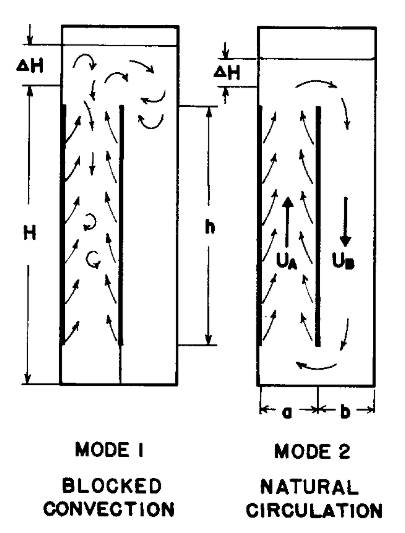
\includegraphics[scale=0.7]{recirculatingsetup.png}
    \caption{Hine's experimental setup for blocked convection and natural circulation \cite{Hine1980}}
    \label{recirculatingsetup}
\end{figure}

Their airlift loop reactor setup provided useful information about the circulation velocity of the liquid phase, which is shown in figure \ref{circulatingvelocity}.

\begin{figure}[H]
    \centering
    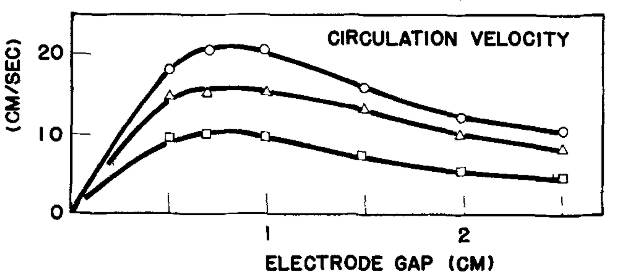
\includegraphics[scale=0.7]{circulatingvelocity.png}
    \caption{circulating velocity as a function of channel gap at different current density \cite{Hine1980}, $\square:i_{av}=750\, \mathrm{A/m^2}, \triangle: i_{av}=2270\, \mathrm{A/m^2},\bigcirc:i_{av}=3720\, \mathrm{A/m^2}$ }
    \label{circulatingvelocity}
\end{figure}


Shah et al. \cite{Jorne1989} also investigated vertical channels with a focus on the mass transfer induced by bubbles. In their study, it was found that the mass transfer in a bubble stirred vertical channel reaches its maximum value at a width of 0.5 cm. Also, vortex at the top region of the channel was found, though the pseudo-turbulence found in other simulation works was not observed.

Abdelouahed et al.\cite{abdelouahed2014hydrodynamics} gave pictures of gas bubble distribution inside a $6 \, \mathrm{mm}$ vertical quiescent channel:




\begin{figure}[H]
    \centering
    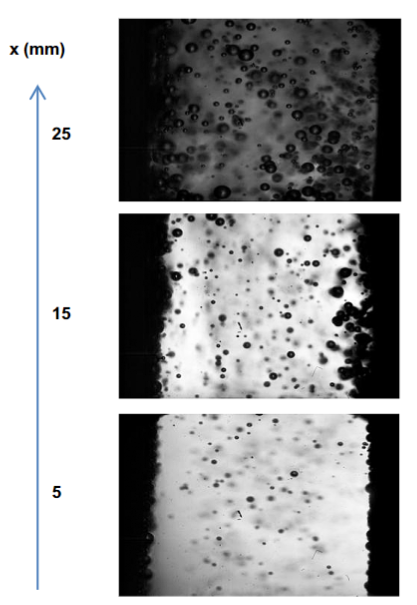
\includegraphics[scale=0.7]{bubblephoto.png}
    \caption{Photo of bubble distribution at three different height $x = 5 \, \mathrm{mm}$, $x = 15 \, \mathrm{mm}$, and $x = 25 \, \mathrm{mm}$ \cite{abdelouahed2014hydrodynamics}, here x refers to height. The width of the channel is 6 mm, and current density is $1000 \, \mathrm{A/m^2}$}
    \label{bubblephoto}
\end{figure}

From the photo, we can see that the gas bubbles are relatively concentrated in the near-wall region. Since this is a quiescent channel, The flow stays laminar.

Riegel et al. \cite{riegel1998role} tested forced circulating flow for water electrolysis with a diaphragm in the middle of the cell and two pumps for both anolyte and catholyte:

\begin{figure}[H]
    \centering
    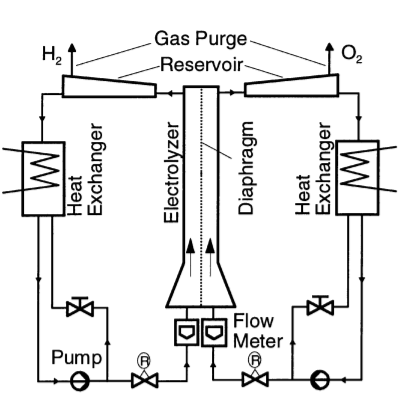
\includegraphics[scale=0.7]{pump.png}
    \caption{Forced circulating flow \cite{riegel1998role}}
    \label{pump}
\end{figure}

In Riegel's study, they found that with high current density, which could produce high gas flux at the electrode surface, backflow could be generated to lower the current density even in a forced flow with high inlet velocity ($\sim 0.5 \, \mathrm{m/s}$). They also provide useful information on gas volume fraction distribution in the channel, though excluding the near-wall region. Based on their data, the volume fraction seems to be more uniformly distributed along the channel width compared with the volume fraction distribution in laminar flow in figure \ref{volumedistributionlag}.

\begin{figure}[H]
    \centering
    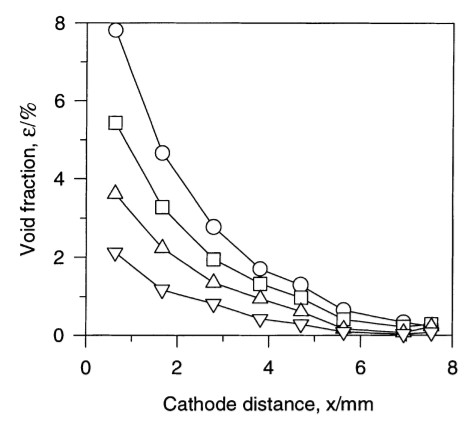
\includegraphics[scale = 0.6]{profile.png}
    \caption{volume fraction profile along the channel width \cite{riegel1998role} under different current density,  $ \nabla: 500\, \mathrm{A/m^2}, \triangle:1500\, \mathrm{A/m^2}, \square: 3250\, \mathrm{A/m^2}, \bigcirc: 6250\, \mathrm{A/m^2}$}
    \label{profile}
\end{figure}

From their experimental data, we can see, the volume fraction does not exceed $0.08$, while in some of the work, it is around $0.4$ \cite{Schillings2015, Dahlkild2001}. Part of the reason could be that their inlet velocity is $0.64 \,  \mathrm{m/s}$, considering their channel width is $8 \, \mathrm{mm}$, we can compute that $\mathrm{Re} \sim 5000$, which is already turbulent. However, it is likely that we still need a more detailed submodel treating the volume fraction at the near-wall region.

\begin{figure}
    \centering
    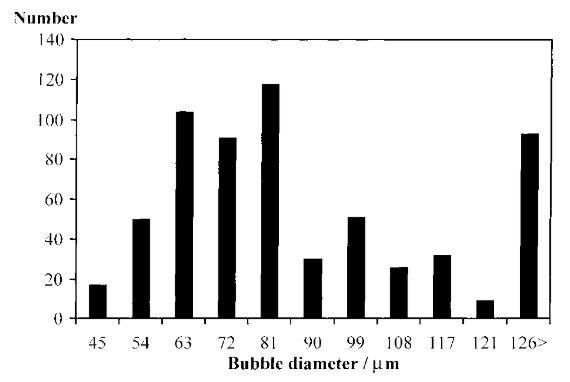
\includegraphics[scale = 0.6]{bubblesizedistribution.png}
    \caption{bubble size distribution in $ 50 \, \mathrm{g/L} $ $ \mathrm{Na_2 SO_4} $ solution under different current density $i_{av} = 2000 \, \mathrm{A/m^2}$ \cite{Boissonneau2000}, the bubbles with diameter larger than $126 \, \mathrm{μ m}$ are mostly oxygen bubbles}
    \label{bubblesize}
\end{figure}

One of the most frequently cited experimental work comes from Boissonneau et al. \cite{Boissonneau2000}. They investigated the bubble induced convection in a vertical channel in a chlorate process and provided the velocity profile along the channel width at several different heights in the channel with the bubble diameter distribution in figure \ref{bubblesize}, which was used widely among many simulations works.

\subsection{Discussion on literature review}

In this section, we discussed a series of literature. The topics mainly involved the volume fraction profile in electrochemical cells, bubble plume thickness, and circulating velocity variation. Most of the experimental works were conducted in quiescent channels or forced flow in vertical channels. 

Although no volume fraction profile data about natural circulating flow were found, we can still gain insights from similar setups, namely forced circulating flow and quiescent flow. From these works, we can know that in laminar flow, bubbles tend to concentrate in the near-wall region, while in turbulent flow bubbles are more uniformly distributed in the channel. This explains why we need a turbulent dispersion force model to describe the influence of turbulence on bubbles. However, it is admitted that we still lack detailed knowledge of the turbulent dispersion force \cite{Rzehak2013}, resulting in most of the model turbulent dispersion model more of a heuristic process than an accurate description.